\section{System Overview}\label{sec-arch}
In this section, we give an overview of the entire architecture of SVC.
\vspace{-.5em}
\subsection{Notation}
Given a database $\mathcal{D}$ which is a collection of relations $\{R_i\}$, a materialized view $S$ is the result of applying the relational expression $S_{def}$ to the database.
We use a multiset algebriac model (a set of elements with corresponding multiplicities) to represent the relations in the database $\mathcal{D}$ and the materialized view $S$.
We denote the multiset of insertions to a relation $R_i$ as $\Delta R_i$ and deletions as $\nabla R_i$.
In this paper, we refer to $\Delta R_i$ and $\nabla R_i$ as ``delta relations".
An update to a relation can be modeled as a deletion and then an insertion.
%In this work, we ignore \textbf{null} types and assume that each tuple in the relation has non-null attribute values.

We look at relation expressions for the view $S_{def}$ composed of the following operators:
\begin{itemize}\vspace{-.45em}
\item $\sigma_{\phi}(R)$: Selection select all tuples $r$ from $R$ that satify the restriction $\phi (r)$ \vspace{-.45em}
\item $\Pi_{a_1,a_2,...,a_k}(R)$: Projection select attributes $\{a_1,a_2,...,a_k\}$ from R \vspace{-.45em}
\item $\bowtie_{\phi (r1,r2)}(R_1,R_2)$: Join select all tuples in $R_1 \times R_2$ that satisfy $\phi (r_1,r_2)$.
\item $\gamma_{e}(R)$\footnote{A special case of this operator is $\delta$ the deduplication operator.}: Aggregation of R grouped by the relational expression $e(R)$.\vspace{-.45em}
\item $R_1 \dot{\cup} R_2$: Multiset union take a union of the two sets incrementing multiplicities.
\item $R_1 \dot{\cap} R_2$: Multiset intersection take an intersection of the set counting multiplicities.
\item $R_1 \dot{-} R_2$: Multiset set difference.
\end{itemize}

\subsection{Formalizing View Maintenance As Data Cleaning}
To apply the algorithms proposed in SampleClean, we need to formalize this problem as a data cleaning problem.
Using the notation defined in the previous section. 
Let $S$ be a materialized view defined by the relational expression $S_{def}$ a composition of operators defined in Section ?? applied to the database $\mathcal{D}$.
Now suppose the relations in $\mathcal{D}$ have been updated with the correponding set of delta relations $U = \{\Delta R_i\} \cup \{\nabla R_i\}$.

$S$ is now \emph{dirty} data, and every query $q$ applied to $S$ will give a dirty result.
As in SampleClean, we take a uniform random sample of ratio $m$ of the dirty data which we call $\hat{S}$.
Based on the operators that we have defined, there are three types of errors that affect $\hat{S}$:
\begin{itemize}
\item A row in $\hat{S}$ needs to be updated.
\item A row in $\hat{S}$ needs to be deleted.
\item To maintain the uniform random sample of ratio $m$ rows need to be added to $\hat{S}$.
\end{itemize}

Based on these data errors, we can define three data cleaning operations to get a cleaned sample of data $\hat{S'}$ (a uniform random sample of ratio $m$ of the up-to-date view $S'$):
\begin{itemize}
\item If an update is needed, update the row.
\item If the row needs to be deleted, delete the row.
\item Add a random sample of ratio $m$ of rows that need to be inserted.
\end{itemize}

The key contribution of this work is efficiently materializing $\hat{S'}$, and using the comparison between $\hat{S}$ and $\hat{S'}$ to correct stale queries on the view.
Of course, in some cases, materializing the sample may require equivalent work to updating the entire view, and we explore the cases in which this technique leads to savings in maintenance costs.

\subsection{Problem Statment}
In this work, we address three distinct problems: (1) query optimization to efficiently find $\hat{S'}$, (2) using $\hat{S}$ and $\hat{S'}$ to calculate an approximate correction for a stale query result, and (3) increased robustness to outliers with outlier indexing.

\subsubsection{Algorithm 1. Efficient Sampling of View Updates}
The input of this algorithm is $\hat{S}$ and the output is $\hat{S'}$.
Define a maintenance plan $\mathcal{M}(\mathcal{D},S_{def},\hat{S},U)$ \footnote{For brevity, we will drop the parameters when not ambiguous.} a maintenance strategy (be it incremental maintenance, full recomputation, or a mix) parametrized by the database, the view definition, the stale sample view, and the set of updates.
A maintenance plan is a relational expression the execution of which returns $\hat{S'}$ by appropriately applying the cleaning operations defined in the previous section using information from the view definition and the updates.

A naive, inefficient approach to this problem would be to materialize $S'$ entirely then select those rows that happen to be in the sample.
Instead, we must exploit the fact that we need not materialize every row and do just enough computation to materialize only the rows in $\hat{S'}$.
This problem defining a sampling operator, which we add to the maintenance plan's query tree, and using relational algebra rules to push this operator as far down the tree as possible.

\subsubsection{Algorithm 2. Query Correction }
Given a query $q$, the stale sample $\hat{S}$, and an up-to-date sample created by the previous procedure $\hat{S'}$.
When $q$ is applied to the full stale view, it gives a stale result of $r$.
We define $c$ a correction, which is a function of $\hat{S}$ and $\hat{S'}$, that gives a corrected result $r-c$.

Like similar restrictions in other sampled-based systems \cite{agarwalknowing}, there are restrictions on the queries $q$ on the view that we can answer. 
In this work, we primarily consider non-nested aggregate queries with simple predicates on a single view:
\begin{lstlisting} [mathescape]
SELECT $f(a)$ FROM View 
WHERE Condition(A);
\end{lstlisting}
We also consider correcting stale non-nested select queries of the following form with simple predicates:
\begin{lstlisting} [mathescape]
SELECT * FROM View 
WHERE Condition(A);
\end{lstlisting}
As with all sample estimates, for the estimates to be meaningful, the predicate should not be too selective.

\subsubsection{Algorithm 3. Outlier Indexing}
We define an outlier index on base relations of the database $\mathcal{D}$.
This index tracks records whose attributes cross some threshold $t$.
For every row in the view that is derived from a record in the outlier index, we ensure that it is incorporated into the sample.
We explore the conditions under which we can make this guarantee.

\subsection{Pratical Use and Implementation}
In implementation, SVC will work in conjunction with existing defered maintenance or re-calculation approaches.
We envision the scenario where materialized views are being refreshed periodically, for example nightly.
While maintaining the entire view throughout the day may be infeasible, sampling allows the database to scale the cost with the performance and resource constraints during the day.
Then, between maintenance periods, we can provide approximately up-to-date query results for some queries.

\subsection{Example Application: Log Analysis}
Without getting into the formal details, to illustrate our system and justify our argument about performance improvements, we use the following running example which is a 
simplified schema of one of our experimental datasets (Figure~\ref{example-1}).
Imagine, we are querying logs from a video streaming company. 
These logs record visits from users as they happen and grow over time.
We have two tables, \tbl{Log} and \tbl{Video}, with the following schema:

\begin{lstlisting}[mathescape]
Log(sessionId$\textrm{,}$ videoId$\textrm{,}$ responseTime$\textrm{,}$ userAgent)
Video(videoId$\textrm{,}$ title$\textrm{,}$ duration)
\end{lstlisting}
These tables are related with a foreign-key relationship between
Log and Video, and there is an integrity constraint that every log
record must link to one video in the Video table.

\begin{figure}[ht!] 
\centering
\vspace{-0.75em}
 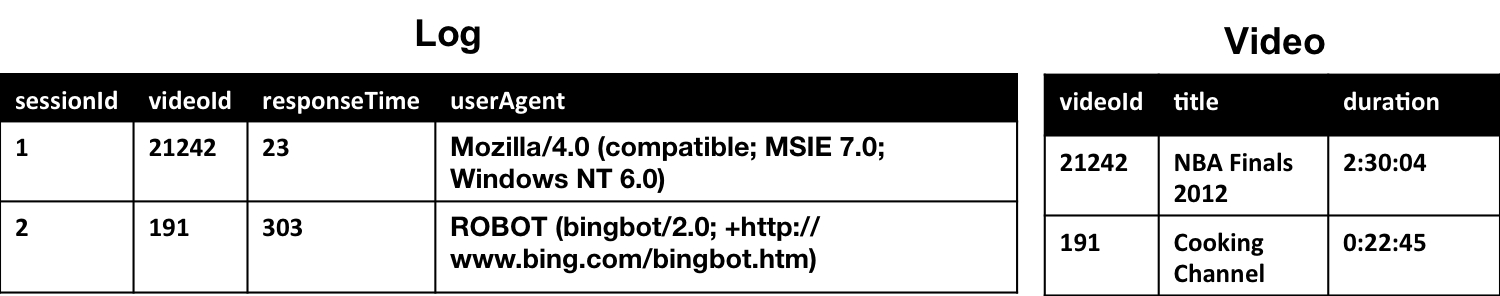
\includegraphics[width=\columnwidth]{figs/sample-clean-example.png}\vspace{-0.25em}
 \caption{A simplified log analysis example dataset. In this dataset, there are two tables: a fact table representing video views and a dimension table representing the videos.\label{example-1}}
\end{figure}

Consider the following example materialized view, which finds a count of the number of times the video's loading latency was greater than 10\% of the duration of the view:

\vspace{0.5em}

\begin{lstlisting} 
SELECT videoId, 
count(1) AS slowResponseTimes 
FROM Log, Video
WHERE Log.videoID = Video.videoID and
	  responseTime > .1*Video.duration
GROUP BY videoId;
\end{lstlisting}

The user wants to know how many videos repeatedly have slow responses.
\begin{lstlisting} 
SELECT COUNT(1)
FROM AggView
WHERE slowResponseTimes > 100;
\end{lstlisting}
Let us suppose the initial query result is $45$.
There now have been new log records inserted into the Log table making the old result stale.
For example, if our sampling ratio is 5\%, that means for 5\% of the videos (distinct videoID's) we refresh stale slowResponseTimes if necessary.
From this sample, we calculate how many new videos changed from a slowResponseTimes of less than 100ms to times greater than 100ms; let us suppose this answer is $2$.
Since our sampling ratio is 5\%, we extrapolate that $40$ new videos throughout the view should now be included in the count.
This means that we should correct the old result by $40$ resulting in the estimate of $85$.

\iffalse
We add the following operator $\eta_{a_1, m}(R)$ which is the \textbf{hash} operator.
For all tuples in R, this operator applies a hash function whose range is $[0,1]$ to attribute $a_1$ and selects those records with hash value less than or equal to $m$.
%We make two assumptions on this hash operator: (1) \emph{independence} there is no expression in $S_{def}$ that is dependent on the hash operator, and (2) \emph{uniformity} over the domain of possible attribute values the \emph{a priori} probability of including any tuple is the same.
Finally, we use the \emph{query tree} representation to analyze $S_{def}$ where we unravel composed relational operators into a tree of expressions.
Each leaf of the tree is a relation and each node is an operator.



\subsection{Semantics of Query Results}
We should note that there is an implicit design tradeoff in the way we formulated this problem.
By sampling the maintenance plans, our approach is very general with respect to supported views.
On the other hand, we are restricted in the types of queries that we can run.
If we were to sample from the delta relations instead, this tradeoff would be flipped. 
We have a further discussion about this subtlty in Section ??.

A important concern of users is what are the semantics and guarantees on their corrected query results.
In Table ??, we list all of the aggregate queries supported by Apache HiveQL present a taxonomy of result semantics for these queries.
We will detail the corrections to these queries in Section \ref{correction}.
\fi